%!TEX root = TDT4265-Summary.tex
\section{Intensity transformations}

%%%%%%%%%%%%%%%%%%%%%%%%%%%%%%%%%%%%%%%%%%%%%%%%%%%%%%%%%%%%
\subsection{Basic functions}
Image intensity levels are defined in the range $[0, L-1]$. $0$ is black, $L$ is white.
\begin{figure}[htbp]
    \centering
    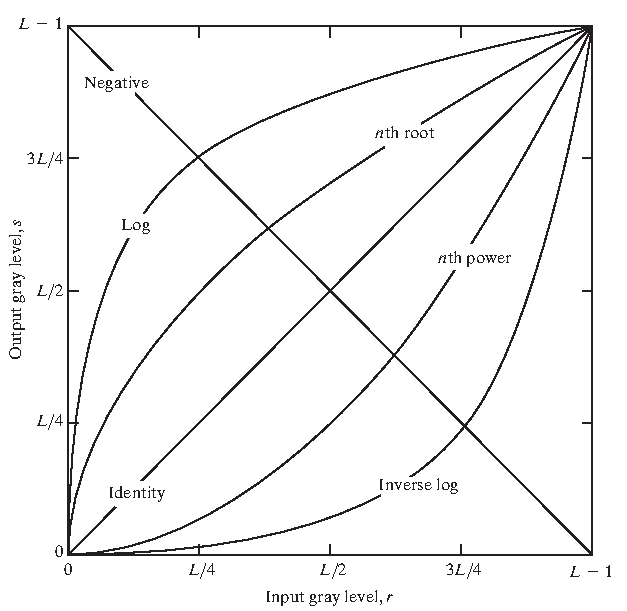
\includegraphics[width=.8\linewidth]{images/basic-transformations}
    \caption{Some basic grey-level transformations}
    \label{fig:basic-transformations}
\end{figure}

\subsubsection{Negative}
Inverts the intensity levels of the image (white becomes black and so on). Enhances details in dark regions.
\begin{equation}
    s = L - 1 - r
\end{equation}

\subsubsection{Log transformation}
Used to expand dark areas and compress bright areas, i.e. give more shadow detail. Good for displaying images with very large dynamic range.
\begin{equation}
    s = c \log(1 + r), \quad r \geq 0
\end{equation}

\subsubsection{Gamma transformation}
Can compress blacks or whites depending on the gamma value. Similar to the log transformation, but more versatile. Many devices have an inherent gamma transform response that can be compensated for by applying the opposite gamma transform. Can be used to improve detail by darkening a washed-out image or brightening a too dark image.
\begin{equation}
    s = c r^\gamma
\end{equation}

\subsubsection{Piecewise linear transformation}
Use a piecewise linear function as the transformation (as opposed to the smooth transformations in Figure \ref{fig:basic-transformations}). Many uses, depending on the function:
\begin{itemize}
    \item Contrast stretching: Increase the dynamic range of the grey levels, similar to a a sigmoid function. (Can also be done with a smooth function.)
    \item Grey-level slicing: Highlight a range of grey-levels. Either leave other values as they are or darken all other values.
    \item Bit-plane slicing: Consider e.g. an 8-bit image to be made of 8 bit `planes'. Extracting one or some of these is called bit-plane slicing. The most significant plane can be extracted to form a binary black or white image, for instance.
\end{itemize}

%%%%%%%%%%%%%%%%%%%%%%%%%%%%%%%%%%%%%%%%%%%%%%%%%%%%%%%%%%%%
\subsection{Histogram processing}

\subsubsection{Histogram equalization}
The cumulative probability density (CPD) of an image is
\begin{equation}
    F(r) = \int_0^r p_r (w) \dif w ,
\end{equation}
which leads to the transformation
\begin{equation}
    s = T(r) = (L-1) F(r).
\end{equation}
$p_r(w)$ is the probability for a pixel to be of intensity $w$. This transformation makes the histogram flat/uniform, which improves contrast by utilizing darks and lights equally much, rather than compressing the image into midtones.

\subsubsection{Histogram matching}
Sometimes you don't want a flat histogram, but a specific, nonflat distribution. Histogram matching is the method of transforming an image so that its histogram matches any given distribution.

\subsubsection{Local histogram processing}
The previous two methods are global, but sometimes a local method is better. This is done by iterating through pixels, looking at and changing the histogram of its neighborhood, and updating the pixel value according to the altered local histogram. An example is histogram equalization for a small moving window.
